\chapter{Pemrograman Dasar}
Tujuan pembelajaran pada pertemuan kedua antara lain:
\begin{enumerate}
\item
Mengenal Jenis Variabel Python
\item
Input dan output user
\item
Operator Dasar
\item
Perulangan
\item
Kondisi
\item
Mengatasi Error
\item
Try Except
\end{enumerate}
Tugas dengan cara dikumpulkan dengan pull request ke github dengan menggunakan latex pada repo yang dibuat oleh asisten IRC. Kode program dipisah dalam folder src NPM.py yang berisi praktek dari masing-masing tugas file terpisah sesuai nomor yang kemudian dipanggil menggunakan input listing ke dalam file latex penjelasan atau nomor pengerjaan. Masing masing soal bernilai 5 dengan total nilai 100.

\section{Teori}
Praktek teori penunjang yang dikerjakan :
\begin{enumerate}
\item
sebutkan jenis-jenis variabel dan jelaskan cara pemakaian variabel tersebut di kode Python
\item
tuliskan bagaimana kode untuk meminta input dari user dan tuliskan bagaimana melakukan output ke layar
\item
Tuliskan operator dasar aritmatika, tambah, kali, kurang bagi, dan 
bagaimana mengubah string ke integer dan integer ke string
\item
Tuliskan dan jelaskan sintak untuk perulangan, jenis-jenisnya contoh kode dan cara pakainya di python
\item
Tuliskan jelaskan cara pakai sintak untuk memilih kondisi, dan bagiamana contoh sintak kondisi di dalam kondisi.
\item
Tuliskan apa saja jenis error yang sering ditemui di python dalam mengerjakan sintak diatas. 
dan bagaimana cara mengatasinya
\item
Tuliskan dan jelaskan cara memakai Try Except.
\end{enumerate}

\section{Ketrampilan Pemrograman}
Buat program di python dengan ketentuan:
\begin{enumerate}
\item
Buatlah luaran huruf yang dirangkai dari tanda bintang, pagar atau plus dari NPM kita.
Tanda bintang untuk NPM mod 3=0, tanda pagar untuk NPM mod 3 =1, tanda plus untuk NPM mod3=2.
Contoh Output : 
\begin{verbatim}
*****    *** ******     *****    ****
*******  *** ***  **    *** **  *****
***  ******* ******     ***  **** ***
***    ***** ***        ***       ***
***     **** ***        ***       ***
\end{verbatim}
NPM sesuai dengan nomor NPM nya.
\item
Buatlah program hello word dengan input NPM yang disimpan dalam sebuah variabel string bernama \textbf{NPM} dan output sebanyak dua dijit belakang NPM, 
contoh NPM : 113040087 maka akan ada output sebanyak 87 dengan tulisan `Hallo, 113040087 apa kabar?'
\begin{verbatim}
Input : 113040087
Output : 
Halo, 113040087 apa kabar? 
Halo, 113040087 apa kabar?
Halo, 113040087 apa kabar?
Halo, 113040087 apa kabar?
Halo, 113040087 apa kabar?
Halo, 113040087 apa kabar?
Halo, 113040087 apa kabar?
Halo, 113040087 apa kabar?
.....87 kali...
\end{verbatim}
\item
Buatlah program hello word dengan input nama yang disimpan dalam sebuah variabel string bernama \textbf{NPM} dan beri luaran output berupa tiga karakter belakang dari NPM sebanyak penjumlahan tiga dijit tersebut, 
\begin{verbatim}
Input : 113040087
Output : Halo, Nama apa kabar? 
Halo, 087 apa kabar?
Halo, 087 apa kabar?
Halo, 087 apa kabar?
Halo, 087 apa kabar?
Halo, 087 apa kabar?
Halo, 087 apa kabar?
Halo, 087 apa kabar?
........15 kali(0+8+7).........
\end{verbatim}
\item
Buatlah program hello word dengan input nama yang disimpan dalam sebuah variabel string bernama \textbf{NPM} dan beri luaran output berupa digit ketiga dari belakang dari variabel NPM, 
\begin{verbatim}
Input : 113040087
Output :
Halo, 0 apa kabar?
\end{verbatim}
\item
\label{digitvar}
(untuk soal no \ref{digitvar} dan selanjutnya wajib menggunakan perulangan dan kondisi) buat program dengan mengisi variabel alfabet dengan nomor npm satu persatu berurut.
Contoh untuk NPM : 113040087 maka,
\begin{verbatim}
a = 1
b = 1
c = 3
e = 0
f = 4
g = 0
h = 0
i = 8
j = 7
\end{verbatim}
Lakukan print NPM lengkap anda menggunakan variabel diatas :

contoh : 113040087
\item
Dari soal no \ref{digitvar}, Lakukan penjumlahan dari seluruh variabel tersebut,
\item 
Dari soal no \ref{digitvar}, Lakukan perkalian dari seluruh variabel tersebut,
\item
Dari soal no \ref{digitvar}, Lakukan print secara vertikal dari NPM anda menggunakan variabel diatas. Contoh:
\begin{verbatim}
1
1
3
0
4
0
0
8
7
\end{verbatim}
\item
Dari soal no \ref{digitvar}, Lakukan print NPM anda tapi hanya dijit genap saja. Contoh:
\begin{verbatim}
48
\end{verbatim}
\item
Dari soal no \ref{digitvar}, Lakukan print NPM anda tapi hanya dijit ganjil saja. Contoh:
\begin{verbatim}
1137
\end{verbatim}
\item 
Dari soal no \ref{digitvar}, Lakukan print NPM anda tapi hanya dijit yang termasuk bilangan prima saja. Contoh:
\begin{verbatim}
37
\end{verbatim}
\end{enumerate}


\section{Ketrampilan Penanganan Error}
Bagian Penanganan error dari script python.
\begin{enumerate}
\item
Tuliskan peringatan error yang didapat dari mengerjakan praktek kedua ini, dan jelaskan cara penanganan error tersebut.
\item
Membuat file 2err.py dan mengisinya dengan script pengisian variabel sebagai string dan pengisian variabel sebagai interger. 
Kemudian jumlahkan antara variabel integer dan string dan tangkap jenis errornya, gunakan try except untuk menunjukkan error tersebut dengan
bahasa indonesia.
\end{enumerate}

\textbf{JAWABAN CHAPTER 2}
\par
\textbf{2.1 Teori}
\begin{enumerate}
\item Penjelasan mengenai variabel dalam dunia pemrograman adalah identitas yang digunakan untuk menampung suatu nilai. Nilai tersebut dapat berubah-ubah tergantung dengan keperluan program. Dapat dikatakan juga bahwa variabel ini seperti tempat penyimpanan yang bisa diisi dengan berbagai data dan (posisi) tempat tersebut bisa kita pindah-pindah sesuai keperluan.
\par
Secara teknis, variabel merujuk kepada suatu alamat di memory komputer. Setiap variabel memiliki nama yang digunakan sebagai identitas untuk menjangkau variabel tersebut.

\begin{itemize}
    \item Jenis-jenis variabel antara lain :
    
    \item Contoh penggunaan variable pada Python :
\begin{figure}[htbp!]
	\centering
	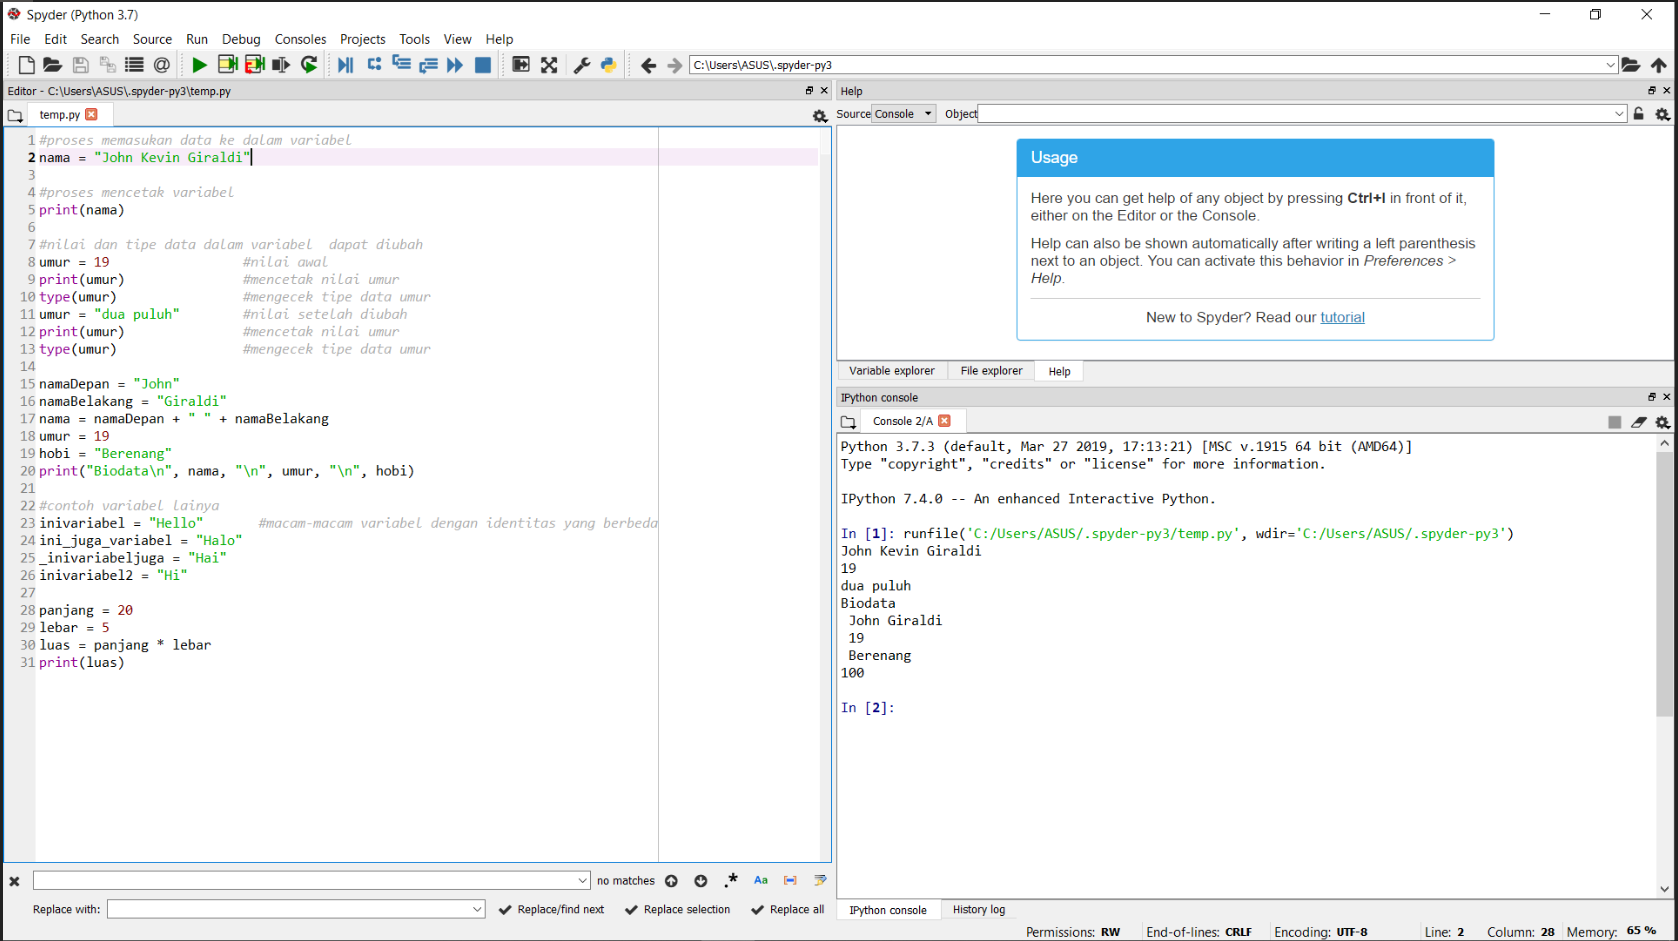
\includegraphics[width=10cm]{figures/cv.PNG}
	\label{fig:gambar}
	\end{figure}
\end{itemize}
\end{enumerate}